\chapter{Positive kernels and the geometry of Stieltjes zeros}\label{ch:zeros}
The derivative tower gives exact spectral coordinates. Its Mellin form
does more: a reciprocal-gamma polynomial becomes a sign-changing kernel
inside a positive Laplace transform. Root preservation bounds the total
number of positive zeros, gamma concentration explains their motion, and
outward rational computation certifies concrete base cases. This chapter
unites the fixed-index zero geometry with the complementary spectral
regime in which the Laurent index grows with the derivative order.

\section{A unified Stieltjes--Lerch derivative family}
\label{zeros:sec:family}

For $a>0$, write
\begin{equation}\label{zeros:eq:laurent}
 \zeta(s,a)=\frac1{s-1}+\sum_{n\geq0}\frac{(-1)^n}{n!}\gamma_n(a)(s-1)^n.
\end{equation}
The superscript in $\gamma_n^{(k)}(a)$ means differentiation $k$ times in $a$. In contrast, $\zeta^{(j)}(s,a)$ denotes differentiation $j$ times in $s$. Set
\begin{equation}\label{zeros:eq:Pk}
 P_k(t)=\prod_{j=1}^k\left(1+\frac tj\right)
       =\sum_{i=0}^k e_i(k)t^i,
 \qquad H_k^{(r)}=\sum_{j=1}^k j^{-r},\quad H_k=H_k^{(1)}.
\end{equation}
We take $H_0^{(r)}=0$.

For $0\leq\rho<1$, define the convergent Lerch coefficients
\begin{equation}\label{zeros:eq:lambda}
 \ell_n(\rho,a)=\sum_{m\geq0}\frac{\rho^m\log^n(a+m)}{a+m}
   =(-1)^n\left.\partial_s^n\Phi(\rho,s,a)\right|_{s=1},
 \qquad
 \Phi(\rho,s,a)=\sum_{m\geq0}\frac{\rho^m}{(a+m)^s}.
\end{equation}
For $k\geq1$ put
\begin{equation}\label{zeros:eq:Dfamily}
 \D_{n,k}^{\rho}(a)=
 \begin{cases}
 \partial_a^k\ell_n(\rho,a),&0\leq\rho<1,\\
 \gamma_n^{(k)}(a),&\rho=1.
 \end{cases}
\end{equation}
Only the derivative family is unified at $\rho=1$: the series defining $\ell_n$ generally diverges there. For $0<\rho<1$ the specialization $a=1$ is directly polylogarithmic,
\begin{equation}
 \ell_n(\rho,1)=\frac{(-1)^n}{\rho}
       \left.\partial_s^n\Li_s(\rho)\right|_{s=1}.
\end{equation}
At $\rho=0$ it is simply $\log^n a/a$.

\begin{proposition}[The classical master identity]\label{zeros:prop:master}
For $k\geq1$, $n\geq0$, and $a>0$,
\begin{equation}\label{zeros:eq:master}
 \gamma_n^{(k)}(a)=(-1)^{n+k}k!n!
     \sum_{i+j=n}e_i(k)\frac{\zeta^{(j)}(k+1,a)}{j!}.
\end{equation}
The same formula with $\Phi(\rho,\cdot,a)$ in place of $\zeta(\cdot,a)$ holds for $\D_{n,k}^{\rho}$ when $\rho<1$.
\end{proposition}
\begin{proof}
The normally convergent defining series gives
$\partial_a^k\zeta(s,a)=(-1)^k(s)_k\zeta(s+k,a)$ first in a right half-plane, and then by meromorphic continuation. Apply it to \eqref{zeros:eq:laurent}, noting that the pole term is independent of $a$. Substituting $s=1+t$ and using $(1+t)_k=k!P_k(t)$ gives
\begin{equation}\label{zeros:eq:mastergen}
 \sum_{n\geq0}\frac{(-1)^n}{n!}\gamma_n^{(k)}(a)t^n
     =(-1)^k k!P_k(t)\zeta(k+1+t,a).
\end{equation}
Coefficient comparison proves \eqref{zeros:eq:master}. For $\rho<1$ the same calculation is justified directly by locally uniform convergence of the Lerch series. This is Coffey's Stirling-number formula in the harmonic/symmetric-function coordinates used by the source draft.
\end{proof}

\begin{definition}[Reciprocal-gamma Appell polynomials]\label{zeros:def:Q}
Define the monic polynomials $Q_n$ by
\begin{equation}\label{zeros:eq:Qgen}
 \frac{e^{xt}}{\Gamma(1+t)}=\sum_{n\geq0}Q_n(x)\frac{t^n}{n!}.
\end{equation}
Set $W_\rho(x)=(1-\rho e^{-x})^{-1}$ for $x>0$ and $0\leq\rho\leq1$.
\end{definition}

Writing $y=x+\gamma$ and $\zeta_r=\zeta(r)$, the first polynomials are
\begin{align}
 Q_0(x)&=1,& Q_1(x)&=y,\notag\\
 Q_2(x)&=y^2-\zeta_2,& Q_3(x)&=y^3-3\zeta_2y+2\zeta_3,\label{zeros:eq:Qsmall}\\
 Q_4(x)&=y^4-6\zeta_2y^2+8\zeta_3y+3\zeta_2^2-6\zeta_4.\notag
\end{align}
They satisfy $Q_n'=nQ_{n-1}$ and the explicit recurrence
\begin{equation}\label{zeros:eq:Qrec}
 Q_{n+1}(x)=(x+\gamma)Q_n(x)
       +\sum_{r=1}^n(-1)^r\binom nr r!\zeta(r+1)Q_{n-r}(x).
\end{equation}
This follows by differentiating \eqref{zeros:eq:Qgen} in $t$ and using
$-\psi(1+t)=\gamma+\sum_{r\geq1}(-1)^r\zeta(r+1)t^r$ near zero.

\begin{theorem}[Appell--Laplace representation]\label{zeros:thm:laplace}
For all $n\geq0$, $k\geq1$, $a>0$, and $0\leq\rho\leq1$,
\begin{equation}\label{zeros:eq:laplace}
 F_{n,k}^{\rho}(a):=(-1)^{n+k}\D_{n,k}^{\rho}(a)
   =\int_0^\infty x^k e^{-ax}W_\rho(x)Q_n(\log x)\dd x.
\end{equation}
The integral and every fixed number of its $a$-derivatives converge locally uniformly for $a>0$, uniformly in $\rho\in[0,1]$.
\end{theorem}
\begin{proof}
The Hurwitz and Lerch Mellin integrals give, for $|t|$ sufficiently small,
\[
 k!P_k(t)\Phi(\rho,k+1+t,a)
   =\frac1{\Gamma(1+t)}\int_0^\infty x^{k+t}e^{-ax}W_\rho(x)\dd x,
\]
where $\Phi(1,s,a)$ means $\zeta(s,a)$ in its convergent half-plane. The cancellation of $\Gamma(k+1+t)$ is the reason for introducing $Q_n$. Extract the coefficient of $t^n$ and apply \eqref{zeros:eq:mastergen}.

For justification, $W_\rho(x)\leq W_1(x)=O(x^{-1})$ at zero and $W_\rho(x)=O(1)$ at infinity, uniformly in $\rho$. On $|t|\leq\eta<k$, the integrand near zero is bounded by a constant times $x^{k-1-\eta}$, and its coefficient derivatives introduce only powers of $|\log x|$. At infinity, a fixed positive lower bound on $a$ supplies exponential domination. Multiplication by any fixed power of $x$ handles the $a$-derivatives. These estimates also prove continuity at $\rho=1$.
\end{proof}

\section{Real-rootedness and a global zero bound}
\label{zeros:sec:zerobound}

\begin{lemma}[A real-root preserving operator]\label{zeros:lem:operator}
If a real polynomial $f$ of degree $n$ has only real roots and $c\neq0$ is real, then $f+cf'$ has only real roots. An inherited root of multiplicity $m$ has multiplicity $m-1$ if $m\geq2$, and every other root of $f+cf'$ is simple. Consequently, after $n-1$ such operators, any real-rooted polynomial of degree $n$ becomes strictly real-rooted.
\end{lemma}
\begin{proof}
Away from the distinct roots $r_i$ of $f$, of multiplicities $m_i$, the new roots solve
\[
 \frac{f'(x)}{f(x)}=\sum_i\frac{m_i}{x-r_i}=-\frac1c.
\]
The left side is strictly decreasing on each complementary interval because its derivative is $-\sum_i m_i/(x-r_i)^2<0$. It has one solution between each consecutive pair of distinct roots and one further solution in the appropriate exterior interval. All these solutions are simple. Factoring at $r_i$ proves the inherited multiplicity assertion, and counting degrees accounts for all roots. Repeating reduces every possible multiple root at each step; new roots never introduce multiplicity.
\end{proof}

\begin{theorem}[Strictly real-rooted reciprocal-gamma polynomials]\label{zeros:thm:Qroots}
For every $n\geq1$, $Q_n$ has exactly $n$ distinct real roots. The roots of $Q_{n-1}$ strictly interlace those of $Q_n$.
\end{theorem}
\begin{proof}
The classical Weierstrass product \cite{zeros:DLMFGamma} is
\begin{equation}\label{zeros:eq:weierstrass}
 \frac1{\Gamma(1+t)}=e^{\gamma t}
       \prod_{m=1}^\infty(1+t/m)e^{-t/m},
\end{equation}
with locally uniform convergence. For a finite product, extracting $n![t^n]$ after multiplication by $e^{xt}$ is equivalent to applying operators $1+\partial_x/m$ and real translations to $x^n$. Lemma~\ref{zeros:lem:operator} therefore proves real-rootedness of each finite-product polynomial. Coefficient convergence and closure of the set of monic real-rooted polynomials prove real-rootedness in the limit.

A limit of simple-rooted polynomials alone would not prove simplicity. To obtain it, remove the first $n-1$ factors $(1+t/m)e^{-t/m}$ from \eqref{zeros:eq:weierstrass}. The Appell polynomial associated with the remaining tail is still real-rooted by the same finite-product argument. Restore the removed factors. The translations preserve multiplicity and commute with the differential operators; the $n-1$ operators $1+\partial_x/m$ make all roots simple by Lemma~\ref{zeros:lem:operator}. Finally $Q_n'=nQ_{n-1}$ and Rolle's theorem give strict interlacing.
\end{proof}

\begin{lemma}[Laplace variation bound, with multiplicity]\label{zeros:lem:variation}
Let $g:(0,\infty)\to\RR$ have exactly $N$ sign changes, with constant nonzero sign between the sign-change points, up to null sets. Suppose all exponentially weighted polynomial moments needed below are absolutely integrable. Its Laplace transform
$G(a)=\int_0^\infty e^{-ax}g(x)\dd x$ is not identically zero and has at most $N$ zeros on $(0,\infty)$, counted with multiplicity.
\end{lemma}
\begin{proof}
For $N=0$ the transform has a fixed strict sign. For $N>0$, choose a sign-change point $x_0$. Multiplying $g$ by $x_0-x$ removes that sign change and introduces no others. The transform of the new function is
\[
 (\partial_a+x_0)G(a)=e^{-x_0a}\frac{\mathrm d}{\mathrm da}\bigl(e^{x_0a}G(a)\bigr).
\]
By induction it has at most $N-1$ zeros. If $G$ has any finite collection of zeros of total multiplicity $M$, Rolle's theorem with multiplicity gives at least $M-1$ zeros of the displayed derivative between the first and last zero, including inherited multiplicities at the endpoints when appropriate. Thus $M\leq N$. This bounds every finite collection, and hence all zeros. The induction hypothesis also says that the transform of the new kernel is not identically zero. If $G$ were identically zero, its displayed transformed derivative would be identically zero as well, a contradiction. This completes the induction including nonvanishing.
\end{proof}

\begin{theorem}[Global bound on positive zeros]\label{zeros:thm:globalzeros}
For every $n\geq0$, $k\geq1$, and $0\leq\rho\leq1$, the function $\D_{n,k}^{\rho}(a)$ has at most $n$ positive zeros, counted with multiplicity. In particular, this holds for $\gamma_n^{(k)}(a)$.
\end{theorem}
\begin{proof}
The factor $x^kW_\rho(x)$ in \eqref{zeros:eq:laplace} is strictly positive. By Theorem~\ref{zeros:thm:Qroots}, $Q_n(\log x)$ has precisely $n$ simple sign changes on $(0,\infty)$. The estimates in Theorem~\ref{zeros:thm:laplace} justify every step of Lemma~\ref{zeros:lem:variation}. The transform is not identically zero: as $a\downarrow0$, scaling $x=u/a$ gives
\begin{equation}\label{zeros:eq:small-a}
 F_{n,k}^{\rho}(a)\sim k!a^{-k-1}\log^n(1/a),
\end{equation}
uniformly in $\rho$, with the convention $\log^0(1/a)=1$. This follows from monicity of $Q_n$ and $W_\rho(u/a)\to1$, using the same integrable bounds after splitting at $u=a$. The variation bound now applies.
\end{proof}

\begin{remark}[The elementary endpoint explains possible multiplicity]
At $\rho=0$ one has
\[
 F_{n,k}^{0}(a)=k!a^{-k-1}\,n![t^n]P_k(t)e^{-t\log a}.
\]
The polynomial in $x=-\log a$ is $\prod_{j=1}^k(1+\partial_x/j)x^n$. It has $n$ real roots counted with multiplicity by Lemma~\ref{zeros:lem:operator}. When $n>k$, the root $x=0$ has multiplicity exactly $n-k$. Thus all zeros cannot be declared simple uniformly in $\rho$ at small $k$. Any uniform simplicity threshold for $n\geq2$ must be at least $n-1$.
\end{remark}

\section{An all-order concentration expansion}
\label{zeros:sec:concentration}

The scale on which the zeros move is $a=ck$, with $c$ bounded away from zero and infinity. Set
\begin{equation}\label{zeros:eq:normalized}
 \Tcal_{n,k}^{\rho}(c)
   =\frac{(-1)^{n+k}(ck)^{k+1}}{k!}\D_{n,k}^{\rho}(ck),
 \qquad h_{n,\rho}(x)=W_\rho(x)Q_n(\log x).
\end{equation}
Let $Y_k$ have gamma density
\[
 \frac{k^{k+1}}{k!}y^k e^{-ky},\qquad y>0.
\]
Then $\EE Y_k=1+1/k$, and \eqref{zeros:eq:laplace} becomes the exact identity
\begin{equation}\label{zeros:eq:expectation}
 \Tcal_{n,k}^{\rho}(c)=\EE\,h_{n,\rho}(Y_k/c).
\end{equation}
The shape is $k+1$, not $k$; the resulting $1/k$ shift matters for the constant term of each zero.

Define polynomials $C_j$ by the formal generating function
\begin{equation}\label{zeros:eq:Cgen}
 \sum_{j\geq0}C_j(z)w^j
   =\exp\left\{\sum_{\ell\geq1}w^\ell
       \left(\frac{z^\ell}{\ell}+\frac{z^{\ell+1}}{\ell+1}\right)\right\}.
\end{equation}
For $C_j(z)=\sum_r c_{j,r}z^r$, use the \emph{normal-ordered} differential operator
\begin{equation}\label{zeros:eq:Aj}
 (A_jh)(x)=\sum_r c_{j,r}x^r h^{(r)}(x).
\end{equation}
This notation does not mean $C_j(x\partial_x)$: the powers of $x$ stand to the left of the derivatives. For example,
\begin{align}
 A_0h&=h,\notag\\
 A_1h&=xh'+\tfrac12x^2h'',\label{zeros:eq:Afirst}\\
 A_2h&=x^2h''+\tfrac56x^3h'''+\tfrac18x^4h^{(4)}.\notag
\end{align}

\begin{theorem}[Uniform complete expansion]\label{zeros:thm:expansion}
Fix $n,J,r\geq0$ and a compact interval $I\subset(0,\infty)$. As $k\to\infty$,
\begin{equation}\label{zeros:eq:expansion}
 \Tcal_{n,k}^{\rho}(c)
   =\sum_{j=0}^J\frac{(A_jh_{n,\rho})(1/c)}{k^j}
          +O_{n,J,r,I}(k^{-J-1}),
\end{equation}
uniformly for $c\in I$ and $0\leq\rho\leq1$, also after any number of $c$-derivatives up to $r$.
\end{theorem}
\begin{proof}
The centered moment generating function is
\[
 \EE e^{z(Y_k-1)}=e^{-z}(1-z/k)^{-k-1}.
\]
For fixed $z$ near zero its logarithm is exactly the convergent expansion
\begin{equation}\label{zeros:eq:mgf}
 \log\EE e^{z(Y_k-1)}
  =\sum_{\ell\geq1}k^{-\ell}
       \left(\frac{z^\ell}{\ell}+\frac{z^{\ell+1}}{\ell+1}\right).
\end{equation}
Consequently the coefficient of $k^{-j}$ in
$\EE(Y_k-1)^m/m!$ is $[z^m]C_j(z)$. For fixed $m$, these moments are finite polynomials in $1/k$, since only finitely many terms of the exponential can contribute to $z^m$. The degree of $C_j$ is at most $2j$.

Here are the estimates needed to turn coefficient comparison into a uniform asymptotic statement. On $1/2\leq y\leq3/2$, all derivatives of $h_{n,\rho}(y/c)$ of any fixed order in $y$ and $c$ are uniformly bounded for $c\in I$ and $\rho\in[0,1]$. Indeed $y/c$ stays in a compact subinterval of $(0,\infty)$ and $1-\rho e^{-y/c}$ is uniformly positive there. Taylor's theorem at $y=1$, through degree $2J+1$, has remainder bounded by $C|y-1|^{2J+2}$. Formula \eqref{zeros:eq:mgf} gives
\[
 \EE|Y_k-1|^{2J+2}=O(k^{-J-1}).
\]
Replacing truncated central moments by full central moments changes the answer only exponentially, as we now verify.

For each fixed derivative order, the functions to be averaged admit bounds
\[
 |\partial_c^u h_{n,\rho}(y/c)|
    \leq C\bigl(y^{-B}+y^B\bigr)(1+|\log y|^n)
\]
for some fixed $B$ and $C$, uniformly in the stated parameters. These follow from $W_1(x)=O(1+x^{-1})$ and its differentiated forms; enlarging $B$ absorbs the logarithm if convenient. For a fixed real exponent $v$,
\[
 \EE\bigl[Y_k^v\mathbf1_{Y_k\notin[1/2,3/2]}\bigr]
 =\frac{\Gamma(k+1+v)}{\Gamma(k+1)k^v}
   \Pr\{Z_{k,v}\notin[1/2,3/2]\},
\]
where $Z_{k,v}$ has shape $k+1+v$ and rate $k$, for all sufficiently large $k$. The prefactor is bounded, and a Chernoff bound obtained from the gamma moment generating function makes the probability $O(e^{-\eta k})$ for some $\eta>0$. The same holds for the finitely many polynomial and inverse-polynomial bounds just used. This proves exponentially small tails for the Taylor remainder and all retained moments.

Taylor expansion in \eqref{zeros:eq:expectation}, followed by \eqref{zeros:eq:mgf}, therefore gives exactly \eqref{zeros:eq:expansion} and the coefficients \eqref{zeros:eq:Aj}. Applying the same argument to $\partial_c^u h_{n,\rho}(y/c)$ proves the stated derivative uniformity. No differentiation of an uncontrolled big-$O$ term is used.
\end{proof}

\begin{remark}[What uniformity does not say]
The constants in Theorem~\ref{zeros:thm:expansion} may depend on $n$ and on the compact $c$-interval. The theorem does not supply estimates uniform when $n$ grows with $k$, nor when $c\downarrow0$ or $c\to\infty$. These are separate problems, especially because the extreme roots of $Q_n$ then control very different scales.
\end{remark}

\section{Exactly \texorpdfstring{$n$}{n} eventual zeros and their locations}
\label{zeros:sec:zerolocations}

Order the Appell roots and define the corresponding slopes by
\begin{equation}\label{zeros:eq:slopes}
 x_{n,1}>x_{n,2}>\cdots>x_{n,n},\qquad
 c_{n,j}=e^{-x_{n,j}},
 \quad 0<c_{n,1}<\cdots<c_{n,n}.
\end{equation}

\begin{theorem}[Uniform eventual zero theorem]\label{zeros:thm:zeroasympt}
For every fixed $n\geq1$ there is an integer $K_n$ such that, for every $k\geq K_n$ and every $\rho\in[0,1]$, $\D_{n,k}^{\rho}$ has exactly $n$ positive zeros, all simple. Number them increasingly as $a_{n,j,k}^{\rho}$. Uniformly in $\rho$,
\begin{equation}\label{zeros:eq:zero2}
 a_{n,j,k}^{\rho}=kc_{n,j}+d_{n,j}(\rho)+O_n(k^{-1}),
\end{equation}
where
\begin{equation}\label{zeros:eq:offset}
 d_{n,j}(\rho)=\frac{c_{n,j}}2
   \left(1+\frac{Q_n''(x_{n,j})}{Q_n'(x_{n,j})}\right)
       -\frac{\rho}{\exp(1/c_{n,j})-\rho}.
\end{equation}
More generally, for every fixed $J\geq0$ there are coefficients $b_{n,j,\ell}(\rho)$ such that
\begin{equation}\label{zeros:eq:zeroall}
 a_{n,j,k}^{\rho}=kc_{n,j}+d_{n,j}(\rho)
   +\sum_{\ell=1}^J b_{n,j,\ell}(\rho)k^{-\ell}
   +O_{n,J}(k^{-J-1}),
\end{equation}
uniformly for $\rho\in[0,1]$. These coefficients are recursively computable from \eqref{zeros:eq:Cgen}.
\end{theorem}
\begin{proof}
The leading term in Theorem~\ref{zeros:thm:expansion} is
\[
 G_0(c,\rho)=W_\rho(1/c)Q_n(-\log c).
\]
Its zeros are exactly the $c_{n,j}$, and its derivative at such a zero is
\begin{equation}\label{zeros:eq:G0prime}
 \partial_cG_0(c_{n,j},\rho)
      =-\frac{W_\rho(1/c_{n,j})}{c_{n,j}}Q_n'(x_{n,j})\neq0.
\end{equation}
Choose disjoint closed intervals around these slopes on whose endpoints $Q_n(-\log c)$ has opposite signs. Since $1\leq W_\rho(1/c)\leq W_1(1/c)$ on their union, the endpoint absolute values are bounded away from zero uniformly in $\rho$. The uniform $J=0$ approximation gives one zero in each interval for all sufficiently large $k$, uniformly in $\rho$. The global bound of Theorem~\ref{zeros:thm:globalzeros} excludes any further zero and, because it counts multiplicity, makes every one of the $n$ zeros simple.

Put $c=c_{n,j}+d/k+O(k^{-2})$. The $k^{-1}$ coefficient of \eqref{zeros:eq:expansion} gives
\begin{equation}\label{zeros:eq:dimplicit}
 d=-\frac{G_1(c_{n,j},\rho)}{\partial_cG_0(c_{n,j},\rho)},
 \qquad G_1(c,\rho)=(A_1h_{n,\rho})(1/c).
\end{equation}
At $x=1/c_{n,j}$, write $Q'=Q_n'(x_{n,j})$ and $Q''=Q_n''(x_{n,j})$. Because $Q_n(\log x)=0$,
\[
 xh'+\tfrac12x^2h''
   =\tfrac12W_\rho(x)(Q'+Q'')+xW_\rho'(x)Q'.
\]
Also
\[
 \frac{W_\rho'(x)}{W_\rho(x)}=-\frac{\rho}{e^x-\rho}.
\]
Substitution in \eqref{zeros:eq:dimplicit} proves \eqref{zeros:eq:offset}.

For completeness, the all-order assertion does not require a convergent power series in $1/k$. Apply Theorem~\ref{zeros:thm:expansion} to one additional order at each step. Substitute a finite ansatz for $c$ into the finite expansion. At every new order the unknown coefficient occurs linearly with the nonzero multiplier \eqref{zeros:eq:G0prime}; hence it is uniquely determined. This derivative is bounded away from zero uniformly in $\rho$. The residual of a truncation, divided by a uniform lower derivative bound on a smaller root interval, bounds the error in the true zero by the mean value theorem. Expanding one order farther than the desired expansion of $a=kc$ gives \eqref{zeros:eq:zeroall} with its stated uniform remainder.
\end{proof}

\subsection{Examples and the first zero}
For $n=1$, $x_{1,1}=-\gamma$ and $c_{1,1}=e^\gamma$. Thus the unique zero of $\gamma_1^{(k)}$ satisfies
\begin{equation}\label{zeros:eq:n1asympt}
 a_{1,1,k}^{1}
   =e^\gamma k+\frac{e^\gamma}{2}
      -\frac1{\exp(e^{-\gamma})-1}+O(k^{-1}).
\end{equation}
The constant term is approximately $-0.4370805068$. At $\rho=0$ the zero is exactly $e^{H_k}$, whose constant term is $e^\gamma/2$; the Lerch kernel therefore changes the constant term, not the slope.
A fully explicit refinement, obtained from Appendix~\ref{zeros:app:nextzero}, is available throughout the deformation. Put $c=e^\gamma$ and $g=\rho/(e^{1/c}-\rho)$. Then, uniformly in $\rho\in[0,1]$,
\begin{equation}\label{zeros:eq:n1third}
 a_k(\rho)=ck+\frac c2-g
   +\frac1k\left\{\frac c{24}+\frac{g(g+1)}c
          -\frac{g(g+1)(2g+1)}{2c^2}\right\}+O(k^{-2}).
\end{equation}
At $\rho=1$, the coefficient of $k^{-1}$ is approximately $0.0288707254211$. At $\rho=0$ it is $c/24$, agreeing with the expansion of the exact zero $e^{H_k}$.


For $n=2$ the roots are $-\gamma\pm\sqrt{\zeta(2)}$, and hence
\begin{equation}\label{zeros:eq:n2slopes}
 c_{2,1}=e^{\gamma-\pi/\sqrt6},\qquad
 c_{2,2}=e^{\gamma+\pi/\sqrt6}.
\end{equation}
The identity $Q_n''(x_j)/Q_n'(x_j)=2\sum_{i\neq j}(x_j-x_i)^{-1}$ gives an alternative expression for every offset entirely in terms of the Appell roots.

\begin{table}[htbp]
\centering\small
\begin{tabular}{rrrr}
\toprule
$n$ & $j$ & slope $c_{n,j}$ & offset $d_{n,j}(1)$\\
\midrule
1&1&1.781072417990&$-0.437080506782$\\
2&1&0.493943487920&$\phantom{-}0.287385687369$\\
2&2&6.422230550060&$-5.227782104747$\\
3&1&0.261424326196&$\phantom{-}0.354674627668$\\
3&2&1.064376550729&$-0.506464646434$\\
3&3&20.305020815096&$-21.208385701520$\\
4&1&0.172347335379&$\phantom{-}0.355378064541$\\
4&2&0.465599872096&$\phantom{-}0.040510911109$\\
4&3&2.062627326998&$-2.178710104429$\\
4&4&60.797835737559&$-70.712693097880$\\
\bottomrule
\end{tabular}
\caption{Numerical evaluations of the exact slope and offset formulas. These decimals are not isolating intervals. The accompanying CSV records zero computations at $k=10,40,160$.}
\label{zeros:tab:slopes}
\end{table}

\subsection{Nonasymptotic information at \texorpdfstring{$n=1$}{n=1}}
\begin{theorem}[Harmonic brackets and monotonicity]\label{zeros:thm:n1brackets}
For each $k\geq1$ and $\rho\in[0,1]$, $\D_{1,k}^{\rho}$ has exactly one positive zero, denoted $a_k(\rho)$. It is simple, and
\begin{equation}\label{zeros:eq:brackets}
 e^{H_{k-1}}<a_k(\rho)\leq e^{H_k}.
\end{equation}
Equality at the upper endpoint occurs exactly when $\rho=0$. The function $\rho\mapsto a_k(\rho)$ is continuous on $[0,1]$ and strictly decreasing. In particular, $a_k(1)<a_k(\rho)<e^{H_k}$ for $0<\rho<1$.
\end{theorem}
\begin{proof}
Normalize the positive density proportional to $x^ke^{-ax}W_\rho(x)$ and write $m(a,\rho)$ for its expectation of $\log X+\gamma$. The sign of $F_{1,k}^{\rho}(a)$ is the sign of $m$. Under an unweighted gamma density of shape $k+1$ and rate $a$, this expectation equals $H_k-\log a$. Weighting by the decreasing function $W_\rho$ lowers the expectation of the increasing function $\log X$; the decrease is strict when $\rho>0$. The elementary covariance identity
\[
 2\Cov(f(X),g(X))
   =\EE\bigl[(f(X)-f(X'))(g(X)-g(X'))\bigr]
\]
for independent identically distributed $X,X'$ justifies this comparison without an external stochastic-order theorem. Hence $m(e^{H_k},\rho)\leq0$, with equality exactly at $\rho=0$.

Alternatively use a gamma density of shape $k$ and rate $a$ and weight it by $xW_\rho(x)$. This weight is strictly increasing, since
\[
 \frac{\mathrm d}{\mathrm dx}\frac{x}{1-\rho e^{-x}}
     =\frac{1-\rho(1+x)e^{-x}}{(1-\rho e^{-x})^2}>0\qquad(x>0).
\]
The unweighted expectation is $H_{k-1}-\log a$, so $m(e^{H_{k-1}},\rho)>0$. A zero exists between the brackets, and Theorem~\ref{zeros:thm:globalzeros} proves uniqueness and simplicity.

For fixed $\rho$, exponential tilting gives
$\partial_a m=-\Cov(\log X,X)<0$. For $\rho_2>\rho_1$, the ratio
\[
 \frac{W_{\rho_2}(x)}{W_{\rho_1}(x)}
    =\frac{1-\rho_1e^{-x}}{1-\rho_2e^{-x}}
\]
is strictly decreasing in $x$. The same covariance comparison therefore gives $m(a,\rho_2)<m(a,\rho_1)$. Together with strict decrease in $a$, this implies $a_k(\rho_2)<a_k(\rho_1)$. Continuity follows from locally uniform dominated convergence in \eqref{zeros:eq:laplace}, uniqueness of the root, and the common compact bracket. No differentiability in $\rho$ at the endpoint $\rho=1$ is assumed.
\end{proof}

\subsection{Propagation and interlacing in the derivative order}
\begin{corollary}[Persistence and rightward interlacing]\label{zeros:cor:interlacing}
Fix $n\geq1$ and $\rho\in[0,1]$. Once $F_{n,k}^{\rho}$ has $n$ distinct positive zeros, the same is true at every larger derivative order. At consecutive such orders,
\begin{equation}\label{zeros:eq:interlacing}
 a_{n,j,k}^{\rho}<a_{n,j,k+1}^{\rho}<a_{n,j+1,k}^{\rho}\quad(1\leq j<n),
 \qquad a_{n,n,k}^{\rho}<a_{n,n,k+1}^{\rho}.
\end{equation}
Thus the unique $n=1$ zero moves strictly rightward for every $k\geq1$.
\end{corollary}
\begin{proof}
Differentiating the integral gives $F_{n,k+1}^{\rho}=-\partial_aF_{n,k}^{\rho}$. Rolle's theorem supplies a zero between each pair of consecutive simple zeros. Also $F_{n,k}^{\rho}(a)\to0$ as $a\to\infty$, and it has a constant nonzero sign after its last zero. There must be a stationary point after that zero: otherwise its nonzero derivative would have constant sign and could not both depart from zero and tend back to zero. Hence there are at least $n$ distinct zeros at the next order. Theorem~\ref{zeros:thm:globalzeros} gives exactly those zeros, all simple, and excludes any zero before the first interval or a coincident zero at an old simple root. Induction proves persistence.
\end{proof}
\section{A recurrence for the next zero coefficient}
\label{zeros:app:nextzero}
For a particular root, abbreviate $c_0=c_{n,j}$ and
$G_m(c,\rho)=(A_mh_{n,\rho})(1/c)$. Suppose
\[
 a_{n,j,k}^{\rho}=kc_0+d+\frac{b_1}{k}+O(k^{-2}).
\]
Taylor expansion of \eqref{zeros:eq:expansion} gives
\begin{equation}\label{zeros:eq:b1}
 b_1=-\frac{\tfrac12\,\partial_c^2G_0(c_0,\rho)d^2
                +\partial_cG_1(c_0,\rho)d+G_2(c_0,\rho)}
               {\partial_cG_0(c_0,\rho)}.
\end{equation}
Here $d$ is \eqref{zeros:eq:offset}, $G_2$ is explicit from \eqref{zeros:eq:Afirst}, and the denominator is nonzero by \eqref{zeros:eq:G0prime}. This is often more usable than a long expanded expression involving several root separations. It also explains why the quantity $k(a-kc_0-d)$ tends to a finite limit. Higher coefficients follow by the same triangular recursion.

\section{The classical half-unit bracket}
For this specialization abbreviate $h_n=h_{n,1}$, and put $t_0=e^{-\gamma}$.

\begin{theorem}[Unique zero and an explicit bracket]\label{half:zero:first}
For every integer $k\geq1$, $\gamma_1^{(k)}(a)$ has a unique positive
zero $a_k$, which is simple.  With $H_0=0$,
\begin{equation}\label{half:zero:half-unit}
 e^{H_{k-1}}<a_k<e^{H_{k-1}}+\tfrac12.
\end{equation}
The zeros are strictly increasing in $k$.  Their asymptotic expansion
starts with
\begin{equation}\label{half:zero:first-asymptotic}
 a_k=e^\gamma\left(k+\tfrac12\right)
                     -\frac1{e^{e^{-\gamma}}-1}+O(k^{-1}).
\end{equation}
Formula~\eqref{zeros:eq:b1} supplies the next coefficient
and an $O(k^{-2})$ remainder.
\end{theorem}
\begin{proof}
The endpoint signs in the endpoint signs and the Laplace representation above
and the bound of one zero prove existence, uniqueness, and simplicity.
To obtain the bracket, normalize the positive density
$t^k e^{-at}/(1-e^{-t})$.  The sign of $F_{1,k}(a)$ is the sign of
$\mathbb E(\log T+\gamma)$ under this density.

Relative to a gamma density of shape $k$ and rate $a$, the tilting
factor is
$r(t)=t/(1-e^{-t})$, which is strictly increasing: its derivative has
numerator $1-e^{-t}(1+t)>0$.  A strictly increasing tilt strictly
increases the expectation of the strictly increasing function
$\log t$.  This elementary fact follows from
\[
 2\operatorname{Cov}(u(X),v(X))
   =\mathbb E[(u(X)-u(Y))(v(X)-v(Y))]>0
\]
for independent $X,Y$ with the same continuous distribution and
strictly increasing $u,v$.  Consequently
\[
 \mathbb E\log T>\psi(k)-\log a
                 =H_{k-1}-\gamma-\log a.
\]
At the zero this gives $a_k>e^{H_{k-1}}\geq1$.

For $a>1/2$, compare instead with a gamma density of shape $k$
and rate $a-1/2$.  The tilting factor is
$s(t)=t/(2\sinh(t/2))$, which is strictly decreasing because
$(t/2)\cosh(t/2)>\sinh(t/2)$.  The covariance inequality reverses:
\[
 \mathbb E\log T<\psi(k)-\log(a-1/2).
\]
Applying it at $a_k>1$ gives $a_k<e^{H_{k-1}}+1/2$.

Finally, at a zero the signed kernel $f(t)$ in
\eqref{zeros:eq:laplace} satisfies $\int e^{-a_kt}f(t)\,dt=0$ and
$(t-t_0)f(t)>0$ except at $t_0$.  Thus
\[
 F_{1,k+1}(a_k)=\int_0^\infty (t-t_0)e^{-a_kt}f(t)\,dt>0.
\]
Since $F_{1,k+1}$ crosses from positive to negative at its unique
zero, $a_{k+1}>a_k$.  The root of $P_1$ is $-\gamma$, so
\eqref{half:zero:first-asymptotic} is Theorem~\ref{zeros:thm:zeroasympt}.
\end{proof}

The interval in \eqref{half:zero:half-unit} is an analytic certificate for
bracketing a unique root, valid even at $k=1$.  Its width is uniformly
$1/2$; no assertion that this is the best possible width is made.
The accompanying computation uses this bracket rather than guessing
an initial zero from a graph.

\begin{figure}[tbp]
\centering
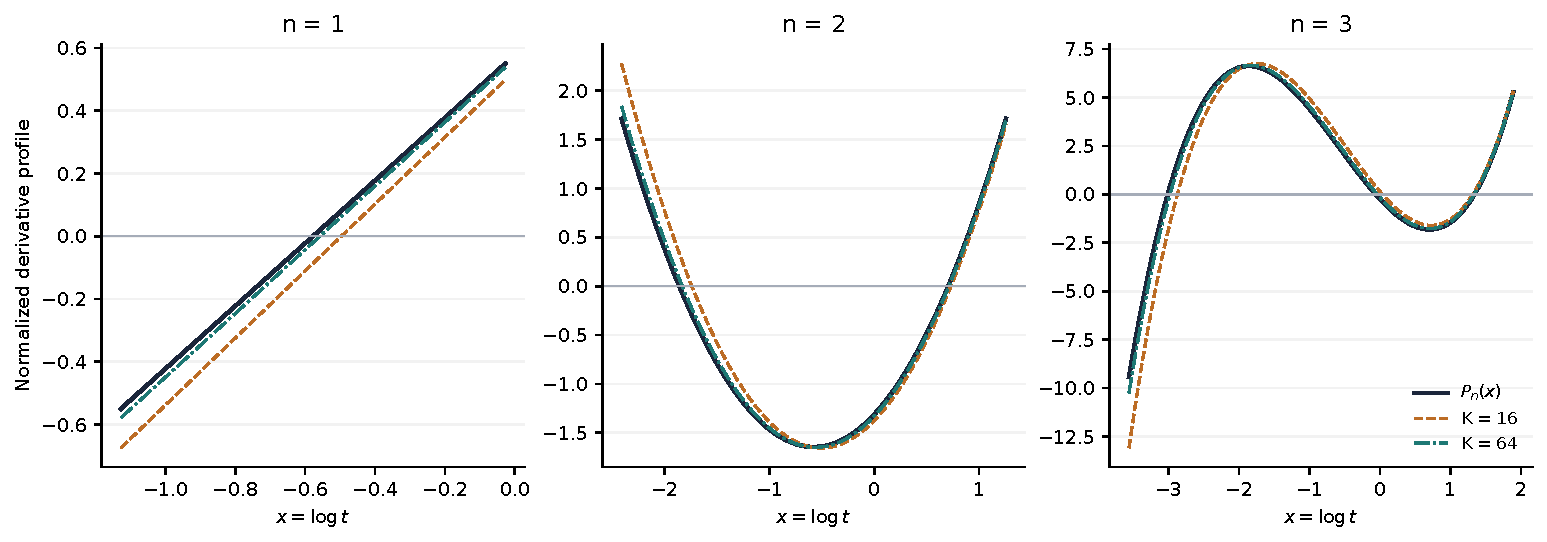
\includegraphics[width=0.98\linewidth]{../reports/corpus-corrections/figures/12-relation-spaces-stieltjes_profiles.pdf}
\caption{Normalized derivative profiles
$(1-e^{-e^x})\mathcal H_{n,K}(e^x)$ approach $P_n(x)$ as $K=k+1$
increases.  The plots illustrate $n=1,2,3$.  Quadrature produces the
curves; Theorems~\ref{zeros:thm:globalzeros} and \ref{zeros:thm:zeroasympt}, rather
than the plots, prove the zero counts and asymptotic completeness.}
\label{half:zero:profile-figure}
\end{figure}

\section{Exact low-index zero counts}
The general theorem proves eventual saturation. At the classical endpoint
$\rho=1$, a finite exact certificate supplies a stronger statement for
$1\le n\le4$ at every $k\ge1$.
Define the sign-preserving normalization
\[
\mathcal V_{n,k}(a)=\frac{a^{k+1}(-1)^{n+k}}{k!}\gamma_n^{(k)}(a).
\]
\subsection{A reproducible Euler--Maclaurin sign certificate}
The finite certificates above can be checked without floating-point special
functions. Put $p=k+1$, and define
\[
R_{n,\ell}(v)=n!\sum_{j=0}^n
 e_{n-j}(\ell)\frac{(-v)^j}{j!}.
\]
The master identity gives the absolutely convergent spectral representation
\[
\mathcal V_{n,k}(a)=\sum_{m\ge0}
 \left(\frac a{a+m}\right)^p R_{n,k}(\log(a+m)).
\]
For positive rational $a$, integers $M,R\ge1$, $A=a+M>1$ and $L=k+2R$,
let
\begin{align*}
\mathcal E_{M,R}={}&\sum_{m=0}^{M-1}
 \left(\frac a{a+m}\right)^p R_{n,k}(\log(a+m))\\
&+\left(\frac aA\right)^p\left[
 \frac Ak R_{n,k-1}(\log A)+\frac12R_{n,k}(\log A)\right]\\
&+\left(\frac aA\right)^p
 \sum_{r=1}^R\frac{B_{2r}}{(2r)!}
 \left(\prod_{j=1}^{2r-1}\frac{k+j}{A}\right)
 R_{n,k+2r-1}(\log A).
\end{align*}
\begin{proposition}[An explicit rational-certifiable remainder]
One has
\begin{align*}
\left|\mathcal V_{n,k}(a)-\mathcal E_{M,R}\right|
&\le\left(\frac aA\right)^p
 \frac{|B_{2R}|}{(2R)!}
 \left(\prod_{j=1}^{2R-1}\frac{k+j}{A}\right)
 \mathcal B_{n,L}(\log A),\\
\mathcal B_{n,L}(v)
&=\sum_{i=0}^{\min(n,L)}\sum_{j=0}^{n-i}
 \frac{n!e_i(L)}{(n-i-j)!L^j}v^{n-i-j}.
\end{align*}
Every factor in the bound is nonnegative.
\end{proposition}
\begin{proof}
Apply Euler--Maclaurin through the $R$th Bernoulli term to the spectral
sum, or equivalently apply it to the Hurwitz series before extracting the
$n$th spectral coefficient. The integral and half-endpoint terms give the
second line of $\mathcal E_{M,R}$. The identity
$(1+u)_k(k+1+u)_{2r-1}=(1+u)_{k+2r-1}$ gives its correction terms.

The periodic Bernoulli remainder has absolute kernel bound $|B_{2R}|$.
After differentiation, bound the absolute value of $R_{n,L}(\log t)$
by $n!\sum_i e_i(L)(\log t)^{n-i}/(n-i)!$ for $t\ge A>1$.
For each $d\ge0$,
\[
\int_A^\infty t^{-L-1}\log^d t\,dt
=\frac{A^{-L}}L\sum_{j=0}^d
 \frac{d!}{(d-j)!L^j}\log^{d-j}A.
\]
The last factor in $(k+1)_{2R}$ cancels the leading $L$ in this
integral. Substitution yields precisely the displayed bound.
\end{proof}

Logarithms of positive rationals have elementary rational enclosures.
Reduce their argument to $1\le y<2$ by a power of two, put
$u=(y-1)/(y+1)$, and use
\[
0\le\log y-2\sum_{j=0}^{T-1}\frac{u^{2j+1}}{2j+1}
\le\frac{2u^{2T+1}}{(2T+1)(1-u^2)}.
\]
The interval verifier uses integer endpoints scaled by $10^{90}$ and
rounds every operation outward. The Bernoulli numbers and $e_i(\ell)$
are exact rationals. A final enclosure lying strictly on one side of
zero is therefore a sign certificate; the proof of the analytic remainder
and the rational arithmetic play separate roles.

The fresh replay verified fourteen base signs for $n\le4$ and sixteen
endpoint signs isolating the unique $n=1$ roots for
$k=1,2,5,10,20,50,100,200$. The endpoint pairs have width $10^{-20}$.
These are global root certificates because the zero-count theorem proves
uniqueness, rather than merely sampled sign changes near a candidate root.


The following enclosures use integer interval arithmetic with outward
rounding, rational logarithm bounds and a proved Euler--Maclaurin remainder.
They have been replayed in this consolidation. The factor $a^{k+1}/k!$
is part of the tabulated value.
\begin{center}
\begin{tabular}{cclc}
\toprule
$n$ & $a$ & Certified enclosure for $\mathcal V_{n,1}(a)$ & Sign\\
\midrule
1 & $1$ & $[0.70738581,\ 0.70738582]$ & $+$\\
1 & $1.5$ & $[-0.20183770,\ -0.20183769]$ & $-$\\
2 & $1$ & $[0.11418372,\ 0.11418373]$ & $+$\\
2 & $1.3$ & $[-0.12008911,\ -0.12008910]$ & $-$\\
2 & $2$ & $[0.45673490,\ 0.45673491]$ & $+$\\
3 & $0.8$ & $[0.16385907,\ 0.16385908]$ & $+$\\
3 & $1.1$ & $[-0.04095264,\ -0.04095263]$ & $-$\\
3 & $1.5$ & $[0.05603756,\ 0.05603757]$ & $+$\\
3 & $2.1$ & $[-0.24542536,\ -0.24542535]$ & $-$\\
4 & $0.8$ & $[0.03897530,\ 0.03897531]$ & $+$\\
4 & $0.94$ & $[-0.00338878,\ -0.00338877]$ & $-$\\
4 & $1.2$ & $[0.02176370,\ 0.02176371]$ & $+$\\
4 & $1.7$ & $[-0.03656822,\ -0.03656821]$ & $-$\\
4 & $2.2$ & $[0.15091738,\ 0.15091739]$ & $+$\\
\bottomrule
\end{tabular}
\end{center}

\begin{corollary}[Saturation at every derivative order for $n\le4$]
For $1\le n\le4$ and every $k\ge1$, $\gamma_n^{(k)}$ has exactly $n$
positive zeros, all simple. They interlace to the right as $k$ increases.
\end{corollary}
\begin{proof}
At $k=1$ each row group gives $n$ sign-changing disjoint intervals, so
there are at least $n$ distinct zeros. The global bound with multiplicity
makes them the only zeros and makes each simple. Persistence and
interlacing follow from Corollary~\ref{zeros:cor:interlacing}.
\end{proof}
This finite certification does not settle every small-$k$ case for
$n\ge5$, and it does not assert saturation at every small order uniformly
in the Lerch deformation.

\section{High parameter derivatives of Stieltjes constants}
\label{spectral:sec:asymptotics}

The parameter-derivative tower admits a useful separation into a
finite polynomial coefficient and an exponentially small spectral
tail. This gives a different asymptotic regime from the frequently
studied limit of a large Stieltjes index with derivative order fixed.
Here the derivative order \(k\) tends to infinity, while the index
\(n\) may grow proportionally to \(\log k\). The resulting profile is
the reciprocal gamma function.

\subsection{An exact spectral expansion}

Fix the Laurent convention
\begin{equation}\label{spectral:eq:stieltjes-convention}
\zeta(s,a)=\frac{1}{s-1}
 +\sum_{n=0}^{\infty}\frac{(-1)^n}{n!}\gamma_n(a)(s-1)^n,
\qquad a>0.
\end{equation}
The superscript \(\gamma_n^{(k)}(a)\) always denotes differentiation
with respect to \(a\), not to the index or the zeta variable. Define
\begin{equation}\label{spectral:eq:coefficient-polynomial}
P_{n,k}(x)=n![z^n]\left(e^{xz}\prod_{j=1}^{k}
                  \left(1+\frac zj\right)\right).
\end{equation}
This is a degree-\(n\) polynomial in \(x\); its coefficients are
rational. In particular \(P_{0,k}=1\) and
\(P_{1,k}(x)=x+H_k\).

\begin{theorem}[Spectral expansion and a finite-tail certificate]
\label{spectral:thm:spectral}
For \(a>0\), integers \(k\ge1\), and \(n\ge0\),
\begin{equation}\label{spectral:eq:spectral}
\frac{(-1)^{n+k}}{k!}\gamma_n^{(k)}(a)
=\sum_{m=0}^{\infty}
 \frac{P_{n,k}(-\log(a+m))}{(a+m)^{k+1}}.
\end{equation}
The series converges absolutely, locally uniformly for \(a>0\).
If the sum is truncated before \(m=M\), where \(b=a+M\ge1\),
then for every real \(0<R<k\) the magnitude of the omitted part is at
most
\begin{equation}\label{spectral:eq:spectral-tail}
\frac{n!}{R^n}\prod_{j=1}^{k}\left(1+\frac Rj\right)
\left(b^{-k-1+R}+\frac{b^{-k+R}}{k-R}\right).
\end{equation}
\end{theorem}

\begin{proof}
The Hurwitz-zeta parameter identity
\[
\partial_a^k\zeta(s,a)=(-1)^k(s)_k\zeta(s+k,a)
\]
follows initially by differentiating its absolutely convergent
Dirichlet series and then by analytic continuation; here
\((s)_k=s(s+1)\cdots(s+k-1)\).
The pole in \eqref{spectral:eq:stieltjes-convention} is independent of \(a\).
Put \(s=1+z\), use
\((1+z)_k=k!\prod_{j=1}^k(1+z/j)\), and compare coefficients.
For \(|z|<k\), the series for \(\zeta(k+1+z,a)\) converges normally.
This gives \eqref{spectral:eq:spectral} and justifies the coefficient
interchange. Alternatively, absolute convergence follows directly
because each summand is a linear combination of
\((a+m)^{-k-1}\log^\ell(a+m)\), \(0\le\ell\le n\).
The parameter identity is also the starting point of
Coffey's all-order formulas~\cite{stieltjes:Coffey}.

On the circle \(|z|=R\), and for \(x\ge b\ge1\),
\[
\left|e^{-z\log x}\prod_{j=1}^k(1+z/j)\right|
\le x^R\prod_{j=1}^k(1+R/j).
\]
Cauchy's coefficient estimate bounds the \(m\)-th omitted summand
by \(n!R^{-n}\prod_j(1+R/j)(a+m)^{-k-1+R}\).
For the positive decreasing power, comparison with its integral gives
\[
\sum_{m=M}^{\infty}(a+m)^{-k-1+R}
\le b^{-k-1+R}+\int_b^\infty x^{-k-1+R}\,dx.
\]
This is \eqref{spectral:eq:spectral-tail}.
\end{proof}

The condition \(b\ge1\) belongs to the stated majorant, rather than to
the exact expansion. It always holds for the tail after the first
term, because then \(b=a+1>1\). The choice of \(R\) can be optimized
for a given \(n,k,M\); there is no need to differentiate a
highly oscillatory numerical representation of \(\gamma_n\).

\subsection{Exact rational enclosures at parameter one}

Write \(\stirling{v}{u}\) for the unsigned Stirling number of the
first kind. The elementary identity
\begin{equation}\label{spectral:eq:stirling-product}
\prod_{j=1}^k(1+z/j)
 =\frac1{k!}\sum_{n=0}^k\stirling{k+1}{n+1}z^n
\end{equation}
turns the first spectral term at \(a=1\) into an exact rational
number.

\begin{corollary}[Rational certificates]\label{spectral:cor:rational}
Let \(k\ge2\), \(n\ge0\), and
\[
e_n(k)=
\begin{cases}
\stirling{k+1}{n+1}/k!,&0\le n\le k,\\
0,&n>k.
\end{cases}
\]
For any integer \(1\le h<k\), set
\begin{equation}\label{spectral:eq:rational-radius}
B_{k,n,h}
=h^{-n}\binom{k+h}{h}
 \left(2^{-k-1+h}+\frac{2^{-k+h}}{k-h}\right).
\end{equation}
Then the following is an exact inclusion between real numbers:
\begin{equation}\label{spectral:eq:rational-inclusion}
\frac{(-1)^{n+k}\gamma_n^{(k)}(1)}{k!\,n!}
\in[e_n(k)-B_{k,n,h},\,e_n(k)+B_{k,n,h}].
\end{equation}
One may take the minimum radius over all \(h=1,\ldots,k-1\).
In particular, the simple choice \(h=1\) gives
\begin{equation}\label{spectral:eq:simple-rational-radius}
B_k=(k+1)\left(2^{-k}+\frac{2^{-k+1}}{k-1}\right),
\end{equation}
independently of \(n\).
\end{corollary}

\begin{proof}
Apply Theorem~\ref{spectral:thm:spectral} with \(a=M=1\), \(b=2\), and
\(R=h\), and divide its bound by \(n!\). The product in that bound is
\(\prod_{j=1}^k(1+h/j)=\binom{k+h}{h}\).
Equation~\eqref{spectral:eq:stirling-product} supplies the center.
All quantities in the resulting endpoints are rational.
\end{proof}

Thus the term \emph{certificate} has its literal meaning here:
integer arithmetic constructs the endpoints, and the proved tail
bound supplies the inclusion. Floating-point agreement is not being
renamed a proof. For example, positivity of an endpoint
\(e_n(k)-B_{k,n,h}\) rigorously proves
\((-1)^{n+k}\gamma_n^{(k)}(1)>0\).
The accompanying script emits centers, radii, and both endpoints
as numerator--denominator pairs, and checks their arithmetic exactly.

\subsection{A uniform coefficient lemma}

The main asymptotic step is an elementary coefficient estimate.
It is convenient to set
\(\fall{n}{j}=n(n-1)\cdots(n-j+1)\) for \(j\le n\), and
\(\fall{n}{j}=0\) for \(j>n\).

\begin{lemma}[Two uniform coefficient terms]\label{spectral:lem:coefficient}
Suppose \(f\) is analytic on a neighborhood of the closed disk
\(|z|\le R\), with \(|f(z)|\le M\) there. Let \(L>0\),
\(n\ge1\), and \(r=n/L<R\). Put
\[
Q_n(L;f)=\frac{n!}{L^n}[z^n]e^{Lz}f(z).
\]
Then
\begin{align}
|Q_n(L;f)-f(r)|
&\le\frac{Mn}{L^2R^2(1-r/R)^3},\label{spectral:eq:coefficient-first}\\
\left|Q_n(L;f)-f(r)+\frac{n}{2L^2}f''(r)\right|
&\le\frac{3Mn}{L^3R^3(1-r/R)^5}.\label{spectral:eq:coefficient-second}
\end{align}
For \(n=0\), \(Q_0(L;f)=f(0)\) exactly.
\end{lemma}

\begin{proof}
Write \(f(z)=\sum_{j\ge0}c_jz^j\). Since \(|c_j|\le MR^{-j}\),
\[
Q_n(L;f)=\sum_{j\ge0}c_j\frac{\fall{n}{j}}{L^j}
\]
is a finite sum, which we compare with the absolutely convergent
Taylor series at \(r\).

For completeness, the needed inequalities remain valid when \(j>n\).
Choose \(j\) independent uniform elements of a set of \(n\) elements.
The probability of no repeated choice is
\(\fall{n}{j}/n^j\), including its value zero when \(j>n\).
For the \(K=\binom j2\) pair-collision events, every event has
probability \(1/n\), and every intersection of two distinct events
has probability \(1/n^2\), even if the pairs share a position.
The union bound and the first two Bonferroni inequalities give
\begin{align*}
0&\le n^j-\fall{n}{j}\le\binom j2 n^{j-1},\\
0&\le\fall{n}{j}-n^j+\binom j2 n^{j-1}
 \le\binom{\binom j2}{2}n^{j-2}.
\end{align*}
At \(j=0,1,2\), the second remainder is zero, so no negative-power
exception is needed. Now use
\[
\sum_{j\ge2}\binom j2 x^{j-2}=(1-x)^{-3},
\qquad
\sum_{j\ge3}\binom{\binom j2}{2}x^{j-3}=3(1-x)^{-5}.
\]
The first inequality gives \eqref{spectral:eq:coefficient-first}.
In the second comparison,
\[
\sum_{j\ge2}c_j\binom j2\frac{n^{j-1}}{L^j}
=\frac{n}{2L^2}f''(r).
\]
This proves \eqref{spectral:eq:coefficient-second}.
\end{proof}

\subsection{The reciprocal-gamma profile}

\begin{theorem}[A joint logarithmic-range asymptotic]\label{spectral:thm:profile}
Fix \(0<a_0\le a_1<\infty\) and \(C>0\). For
\(a\in[a_0,a_1]\), put
\[
L=\log(k/a),\qquad r=\frac nL,\qquad
g(r)=\frac1{\Gamma(1+r)},\qquad
\rho=\frac{a_1}{a_1+1}<1.
\]
Uniformly over integers \(0\le n\le CL\), as \(k\to\infty\),
\begin{equation}\label{spectral:eq:uniform-profile}
\frac{(-1)^{n+k}a^{k+1}\gamma_n^{(k)}(a)}{k!\,L^n}
=g(r)-\frac{n}{2L^2}g''(r)
 +O_{a_0,a_1,C}\left(\frac n{L^3}+k^{C+1}\rho^k\right).
\end{equation}
Equivalently, the two displayed terms are
\begin{equation}\label{spectral:eq:profile-polygamma}
\frac1{\Gamma(1+r)}
\left[1+\frac{n}{2L^2}
 \left\{\psi^{(1)}(1+r)-\psi(1+r)^2\right\}\right].
\end{equation}
The formula includes \(n=0\), for which the first spectral term is
exactly one. In particular, if \(n/\log(k/a)\to c\ge0\) in a bounded
range, then the left side of \eqref{spectral:eq:uniform-profile} tends to
\(1/\Gamma(1+c)\).
\end{theorem}

\begin{proof}
Separate the \(m=0\) term of \eqref{spectral:eq:spectral}. Its generating
function factors as
\[
e^{-z\log a}\prod_{j=1}^k(1+z/j)=e^{Lz}f_k(z),
\qquad
f_k(z)=k^{-z}\prod_{j=1}^k(1+z/j).
\]
The gamma product gives
\[
f_k(z)=\frac{\Gamma(k+1+z)}
 {\Gamma(k+1)k^z\Gamma(1+z)}
      =g(z)e^{D_k(z)}.
\]
On \(|z|<k+1\), define the analytic function
\begin{equation}\label{spectral:eq:Dk}
D_k(z)=z(H_k-\log k-\gamma)
 +\sum_{\ell=2}^{\infty}
   \frac{(-1)^\ell z^\ell}{\ell}
       \bigl(\zeta(\ell)-H_k^{(\ell)}\bigr).
\end{equation}
The factorization follows first on a small disk from the
Weierstrass product and then throughout \(|z|<k+1\) by analytic
continuation. Defining \(D_k\) by its series avoids taking the
logarithm of \(g\) at its zeros.

The elementary bounds
\[
0<H_k-\log k-\gamma<\frac1{2k},\qquad
\sum_{j>k}j^{-2}\le\frac1k
\]
imply, for \(|z|\le R<k+1\),
\begin{equation}\label{spectral:eq:Dk-bound}
|D_k(z)|\le\frac{R}{2k}
   +\frac{R^2}{2k(1-R/(k+1))}.
\end{equation}
Indeed, for \(\ell\ge2\), bound the tail of \(\zeta(\ell)\) by
\((k+1)^{2-\ell}/k\), and use \(1/\ell\le1/2\).
Consequently \(f_k\) is uniformly bounded on every fixed disk,
\(f_k-g=O_R(k^{-1})\), and Cauchy's estimate gives
\(f_k''-g''=O_C(k^{-1})\) on \([0,C]\).
The same estimate with \(R=r\), or the real product, also gives the
slightly sharper
\[
f_k(r)-g(r)=O_C(r/k)\qquad(0\le r\le C).
\]
It is this factor \(r\) that preserves the exact \(n=0\) first term.

Choose \(R=C+1\) in Lemma~\ref{spectral:lem:coefficient}. For \(n\ge1\)
the normalized first spectral term is
\[
Q_n(L;f_k)
=f_k(r)-\frac{n}{2L^2}f_k''(r)+O_C(n/L^3).
\]
Replacing \(f_k\) by \(g\) costs
\(O_C(n/(kL)+n/(kL^2))\), which is absorbed in \(O(n/L^3)\)
because \(L^2\le k\) for all sufficiently large \(k\), uniformly
on the compact parameter interval.

It remains to control the other spectral terms. Apply
\eqref{spectral:eq:spectral-tail} with \(M=1\), and multiply the bound by
\(a^{k+1}/L^n\). The result is
\[
\frac{n!}{(RL)^n}\prod_{j=1}^k(1+R/j)
\left(\frac{a}{a+1}\right)^{k+1}(a+1)^R
\left(1+\frac{a+1}{k-R}\right).
\]
The first factor is at most one: for \(n\ge1\), use
\(n!\le n^n\) and \(n/L\le C<R\); for \(n=0\), it is one by
convention. The product is \(O_R(k^R)\), as follows already from
\eqref{spectral:eq:Dk-bound} at \(z=R\).
The remaining factors are uniformly bounded apart from
\((a/(a+1))^{k+1}\le\rho^{k+1}\). Thus the normalized tail is
\(O_{a_0,a_1,C}(k^{C+1}\rho^k)\). The case \(n=0\) follows
directly from \(P_{0,k}=1\).
Finally,
\(g''(r)=g(r)\{\psi(1+r)^2-\psi^{(1)}(1+r)\}\).
\end{proof}

\begin{corollary}[A uniform eventual sign]\label{spectral:cor:sign}
For every compact interval \([a_0,a_1]\subset(0,\infty)\) and
every \(C>0\), there is \(k_0\) such that
\[
(-1)^{n+k}\gamma_n^{(k)}(a)>0
\]
for all \(k\ge k_0\), \(a\in[a_0,a_1]\), and integers
\(0\le n\le C\log(k/a)\).
\end{corollary}

\begin{proof}
The continuous function \(g\) is strictly positive on \([0,C]\),
so its minimum there is positive. Both the displayed correction
and the remainder in Theorem~\ref{spectral:thm:profile} tend uniformly to zero.
The other factors in the normalization are positive.
\end{proof}

The corollary is restricted to its stated range. It gives no sign
theorem when \(n\) grows arbitrarily quickly compared with \(\log k\).
For a concrete finite pair \(n,k\) at \(a=1\), the rational interval
in Corollary~\ref{spectral:cor:rational} is a separate, effective certificate.

\begin{figure}[tbp]
\centering
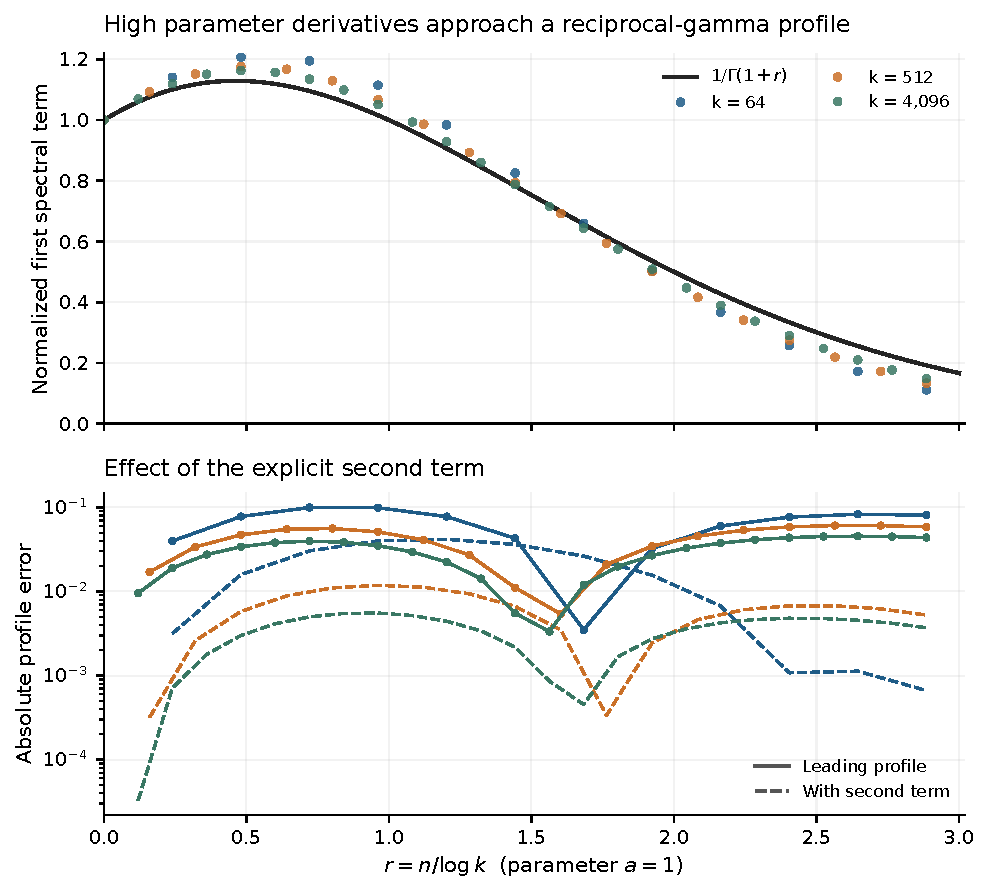
\includegraphics[width=\textwidth]{../reports/rational-grid-distribution-ranks/figures/10-exact-structure-derivative-profile.pdf}
\caption{The reciprocal-gamma profile at \(a=1\).
The first spectral term is computed from the elementary-symmetric
coefficient recurrence; its rigorously bounded spectral error is
smaller than the plotted resolution.
The lower panel compares its deviation from the limiting profile
with its deviation after the explicit second term is included.
These plotted arithmetic evaluations are floating point; the separate
rational certificates do not depend on them.}
\label{spectral:fig:profile}
\end{figure}

\subsection{Fixed-index expansions and the classical mechanism}

For a fixed \(n\), it is also useful to retain the polynomial in
\(L=\log(k/a)\). Define Appell polynomials
\[
A_n(L)=n![z^n]\frac{e^{Lz}}{\Gamma(1+z)}.
\]
The first few are
\begin{align*}
A_0(L)&=1,\\
A_1(L)&=L+\gamma,\\
A_2(L)&=(L+\gamma)^2-\zeta(2),\\
A_3(L)&=(L+\gamma)^3-3\zeta(2)(L+\gamma)+2\zeta(3).
\end{align*}
The standard gamma-ratio expansion~\cite{hstruct:DLMF} gives, uniformly on
fixed \(z\)-disks,
\[
e^{D_k(z)}=
1+\frac{z+z^2}{2k}
 +\frac{3z^4+2z^3-3z^2-2z}{24k^2}+O(k^{-3}).
\]
Consequently, for fixed \(n\ge1\) and \(a\) in a compact positive
interval,
\begin{align}
\frac{(-1)^{n+k}a^{k+1}\gamma_n^{(k)}(a)}{k!}
={}&A_n(L)
 +\frac{nA_{n-1}(L)+n(n-1)A_{n-2}(L)}{2k}\notag\\
&+O_n\left(\frac{(1+L)^{n-1}}{k^2}\right)
 +O_{a_0,a_1,n}(k^2\rho^k).
\label{spectral:eq:fixed-index}
\end{align}
Terms with a negative Appell index are omitted.
To see the stated polynomial error, note that the analytic
remainder after the first correction vanishes at \(z=0\);
its coefficient convolution with \(e^{Lz}g(z)\) therefore has
degree at most \(n-1\) in \(L\). For \(n=0\) the first term is
exact and only the spectral error remains.
Higher powers of \(k^{-1}\) follow by the same coefficient procedure.
For example the \(k^{-2}\) numerator is
\[
\frac1{24}\left(
3\fall{n}{4}A_{n-4}
+2\fall{n}{3}A_{n-3}
-3\fall{n}{2}A_{n-2}
-2nA_{n-1}\right).
\]

At \(a=1\), \eqref{spectral:eq:stirling-product} identifies the first spectral
term with first-kind Stirling numbers. These are also the cycle-count
coefficients of permutations. The reciprocal-gamma factor is thus a
classical mechanism, closely related to mod-Poisson asymptotics
\cite{spectral:KowalskiNikeghbali}. The contribution to this programme is the
explicit spectral transfer, the uniform second coefficient estimate,
and the exact rational enclosure, not a claim that the
reciprocal-gamma phenomenon itself is new.
